\documentclass[../main]{subfiles}
\ifSubfilesClassLoaded{
    \dominitoc
    \tableofcontentsfile
    \pagenumbering{arabic}
    \setcounter{page}{1}
	\setcounter{chapter}{2}
	\addbibresource{../Biblio/biblio.bib}
}{}

\begin{document}
\chapter{Analyse du mécanisme de relaxation}\label{chap:relaxation}
\graphicspath{{./},{07-Relaxation/}}

\minitoc

\section{Introduction}

\subsection{Du calcul cellulaire au calcul à l'échelle d'une carte}

Le processus de relaxation que nous avons défini au chapitre précédent dans l'algorithme CxSOM est une méthode originale pour construire des connexions bidirectionnelles entre cartes.
Dans ce chapitre, nous chercherons à observer le comportement de la relaxation et notamment sa convergence dans les cartes de l'architecture CxSOM. 
Avant cela, nous nous intéressons à son inspiration biologique et pourquoi il reste proche des architectures de cartes cellulaires développées précédemment dans l'équipe \cite{khouzam_neural_2014,menard05}, qui ont inspiré ces travaux.

Dans ces modèles d'architectures, le processus dynamique d'apprentissage s'appuyait sur des champs neuronaux dynamiques couplés (DNF), qui remplacaient la recherche de BMU.
Les DNF, introduits en \cite{Amari1977DynamicsOP} permettent de modéliser à gros grains l'activité spatiotemporelle d'une population de neurones impulsionnels. 
Au lieu de s'intéresser à l'activité d'un seul neurone, tel que son taux de décharge, le modèle des DNF calcule un potentiel $u(x,t)$ en un ensemble de positions continues $x$ à un temps $t$, réagissant à un stimulus d'entrée $s(x,t)$. Les positions $x$ s'étendent sur l'espace des caractéristiques d'entrée et représentent une valeur dans cet espace. Ainsi, un DNF réagissant à un stimulus 1D est en une dimension, etc.
L'activation du DNF est ensuite une approximation du taux de décharge moyen du champ de neurones à chaque position $x$. Par exemple, l'évolution du potentiel $u$, en temps continu sur un espace $x$ en une dimension s'exprime par l'équation différentielle~:

\begin{equation}\label{eq:DNF}
	\tau \frac{\partial u(x,t)}{\partial t} = - u(x,t) + + s(x,t) + h + \int_{-\infty}^{\infty} \omega(x - y)g(u(y,t))dy 
\end{equation}

\begin{figure}
	\centering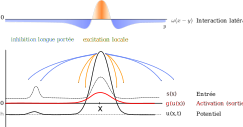
\includegraphics[width=0.9\textwidth]{DNF.pdf}
	\caption{Schéma des éléments intervenant dans le calcul du potentiel $u$ du DNF~\ref{eq:DNF}, ici pour un signal d'entrée $s(x)$ en une dimension, constant dans le temps.
	Le potentiel $u$ du DNF évolue grâce aux interactions entre les positions $x$ par l'interaction latérale $\omega$.
	L'évolution amène toute l'activation $g(u(x))$ autour d'un seul point, qui se situe au maximum de $s(x)$~: le maximum local de gauche n'a pas de représentation dans l'activation totale, à cause des connexions inhibitrices.
	Ce DNF implémente ainsi un mécanisme de Winner Take All. \label{fig:DNF}
	}
\end{figure}

L'évolution du potentiel en chaque point $x$ dépend ainsi de l'état d'activation de tout le DNF, intégré sur les positions. $g(u(y))$ est une fonction sigmoïde centrée en zéro représentant l'activation à une position $y$, de telle sorte qu'une position $y$ du champ n'est prise en compte dans l'interaction générale, que si son potentiel dépasse un certain seuil d'activation. $g(u(x,t))$ correspondra également à la valeur utilisée comme sortie du DNF.
$\omega(x-y)$ est un terme d'interaction latérale, en général une différence de gaussiennes, rendant le voisinage proche de $x$ \emph{excitateur}~: son activation renforce le potentiel $u(x,t)$, tandis que le voisinage à plus longue distance est inhibiteur. 
Ensuite, $s(x,t)$ est le signal d'entrée du DNF, et $h$ est un niveau de repos.
Le calcul du potentiel $u$ d'un DNF sur un stimulus d'entrée résulte en la formation de bulles d'activités dans les zones ou le signal d'entrée est élevé, implémentant un mécanisme de Winner Take All.
Ces grandeurs sont illustrées en figure~\ref{fig:DNF} pour un exemple sur une entrée $s(x)$ 1D constante dans le temps.

Les DNF ont plusieurs applications possibles en fonction des paramètres choisies, comme le filtrage de bruit ou le suivi d'une cible positionnée en $x$.
Le calcul du potentiel s'appuie sur tout le champ d'activation, mais les éléments qui ont vraiment une influence sont situés sur un voisinage de $x$ en chaque point. Les calculs permettant ce mécanisme Winner Take All peuvent ainsi être considérés comme cellulaires.
Des DNF réagissant à plusieurs signaux d'entrée $s_i(x)$ peuvent être couplés en des architectures dynamiques, exhibant des mécaniques complexes, présentées par exemple en \cite{Fix2011ADN, Sandamirskaya2014DynamicNF}.
Ces travaux montrent que le couplage de DNF permet d'envisager des comportements autonomes au sein de structures de DNF, et non une seule réaction à l'entrée $s$.
La construction d'architectures de cartes auto-organisatrices cellulaires en~\cite{khouzam_neural_2014,menard05} utilise des DNF couplés entre cartes afin de choisir le BMU d'une carte, c'est à dire l'unité dont le poids va être mis à jour.
Les architectures de cartes proposées dans ces travaux ajoutent finalement un mécanisme d'apprentissage aux DNF, qui sont à la base un processus dynamique réagissant aux entrées. 
Les DNF apportent quant à eux le calcul cellulaire manquant aux cartes auto-organisatrices classiques pour réaliser des calculs au niveau du neurone et non de la carte.

La recherche de BMU d'une carte de Kohonen implémente également un mécanisme de Winner Take All, mais dont le calcul est centralisé à l'échelle de la carte grâce au calcul de l'activation des neurones.
Ce calcul centralisé nécessite moins de ressources de calcul que le calcul des DNF, qui s'appuie sur la résolution numérique d'une équation différentielle.

Dans le même esprit que l'utilisation d'une activation chez Kohonen pour trouver le BMU au lieu d'un mécanisme cellulaire, l'algorithme de relaxation que nous avons proposé cherche à conserver un processus dynamique de recherche de BMU mais en plaçant les calculs à l'échelle d'une carte. 
Le choix d'un BMU $\bmu$ dans une carte auto-organisatrice par un $\argmax$ équivaut à la génération d'une bulle d'activité centrée en $\bmu$ dans un DNF. 
Le processus dynamique de relaxation que nous utilisons dans le modèle CxSOM se rapproche ainsi des mécanismes réalisés dans les DNF couplés, mais en remplacant le processus cellulaire réalisé dans une carte par le calcul d'activité et le choix du BMU. Le couplage entre les activités des cartes reste par contre un processus dynamique.
Ce choix nous a permis de simplifier grandement les calculs réalisés au sein d'une carte afin d'envisager d'étudier facilement des grandes architectures de cartes, tout en conservant une proximité avec une version cellulaire des cartes auto-organisatrices.

Dans notre modèle, le mécanisme de relaxation cherche à la fois à trouver un BMU dans chaque carte, c'est-à-dire une position à laquelle l'activité est maximale, et joue le rôle d'interface entre cartes en utilisant la position du BMU dans les cartes voisines pour le calcul d'activité. 

\subsection{Problématique du chapitre}

Dans ce chapitre, nous nous intéressons à la relaxation en tant que mécanisme d'interface entre cartes.
Nous chercherons d'abord à décrire formellement l'algorithme de relaxation proposé dans le modèle CxSOM afin de pouvoir mieux analyser et représenter sa dynamique. 
Nous nous demanderons notamment si la relaxation est équivalente, comme dans une carte simple, à une recherche de maximum d'activation et expliciterons les propriétés de convergence qu'on attend de l'algorithme de relaxation pour pouvoir le considérer comme une recherche de \og Best Matching Unit \fg{}. Nous attendons notamment que la recherche de BMU converge et que le point de convergence soit unique.
Le comportement de la relaxation dépend complètement des configurations des poids externes et contextuels des cartes de l'architecture. Ces configurations de poids résultent d'un processus de mise à jour et n'ont pas de formulation analytique. Ce chapitre n'a pas pour but d'apporter une preuve de convergence. 
Les formalisations que nous présentons permettent de mieux comprendre les mécanismes en jeu lors de la relaxation et de comprendre les tracés du comportement sur les exemples présentés en section~\ref{sec:relax_expe}.

\section{Formalisation de l'algorithme de relaxation}

La recherche du BMU par relaxation dans l'architecture CxSOM se traduit par une recherche du maximum des activations de chacune des cartes de l'architecture.
La relaxation est une heuristique de recherche de ce maximum.
Nous formalisation dans cette section la relaxation et formulons le problème d'optimisation qu'elle cherche à résoudre. 
Nous introduisons ainsi des notations plus détaillées qui nous permettront d'observer les quantités relatives à l'évolution de la relaxation en section suivante.

\subsection{Formulation de l'évolution des BMUs lors de la relaxation}\label{sec:formulation_suite}

La relaxation définie dans le modèle est une recherche de maximum par déplacements de $(p\m{1},\cdots, p\m{n})$l'espace des positions de toutes les cartes.

Nous définissons cette recherche comme une suite $(\mathbf{\bmu})_\tau = (\bmu\m{1}_\tau,\cdots,\bmu\m{n}_\tau)$ dont nous voulons exprimer ici l'équation d'évolution.

Définissons d'abord la suite $\hat{p}\m{i}_\tau$, qui correspond à la position maximisant l'activité globale de la carte $i$ à l'instant $\tau$~:
\begin{equation}
\begin{gathered}
\hat{p}\m{i}_{\tau} = \argmax_p(a_g\m{i}(p,\bmu\m{i_0}_\tau, \cdots \bmu\m{i_K}_\tau))\\
 i_0, \cdots i_K \: \text{indices des cartes nourrissant la carte $i$}.
\end{gathered}
\label{eq:pstar}
\end{equation}

L'équation d'évolution de la suite $(\mathbf{\bmu})_\tau$ s'écrit alors à partir de $\hat{p}_\tau$:

\begin{equation}
\bmu\m{i}_{\tau+1} = 
\begin{cases}
\bmu\m{i}_{\tau} + sgn(\hat{p}\m{i}_{\tau} - \bmu\m{i}_{\tau}) \times \Delta \; & \text{si $\hat{p}\m{i}_{\tau} - \bmu\m{i}_{\tau} > \Delta$ } \\
\hat{p}\m{i}_{\tau} \; \text{sinon}	
\end{cases}
\label{eq:evolution}
\end{equation}

$a_g\m{i}$ est une fonction des poids de la carte $\w\ext\m{i}, \w\cont\m{i}$ et de son entrée externe $\inpx\m{i}$. 
Lors du processus de relaxation, les poids et l'entrée $\inpx\m{i}$ restent fixes. 
Le calcul de $a_g\m{i}$ à l'instant $\tau$ ne dépend sonc pas de $\tau$.
Pour toute carte $i$, $\hat{p}\m{i}_{\tau}$ dépend uniquement de $(\bmu\m{i_0}_\tau, \cdots \bmu\m{i_K}_\tau)$. 
En posant $f\m{i}$ toute la partie droite de l'équation \ref{eq:evolution}, on peut donc écrire~:

\begin{equation}
\forall i, \; \bmu\m{i}_{\tau +1} = f\m{i}(\bmu\m{1}_\tau,\cdots,\bmu\m{n}_\tau)
\label{eq:fonction}
\end{equation}

Soit, pour l'ensemble des composantes: 
\begin{equation}
\mathbf{\bmu}_{\tau+1} = \mathbf{f}(\mathbf{\bmu}_\tau)
\end{equation}

Si $(\mathbf{\bmu})_\tau$ converge, alors elle converge vers un point fixe de la fonction $f$, soit une position $\mathbf{\bmu}$ vérifiant~:
\begin{equation}
\mathbf{\bmu} = \mathbf{f}(\mathbf{\bmu})
\label{eq:suite}
\end{equation}

Rien ne garantit que des points fixes existent ni que la suite converge~: $\mathbf{f}$ dépend de l'organisation des poids externes et contextuels de chaque carte, qui sont aléatoirement répartis au début de l'apprentissage.
Pour des poids $\w$ quelconques, il n'existe d'ailleurs généralement pas de point fixe.

Enfin, que l'évolution de la suite $(\mathbf{\bmu})_{\tau}$ dépend de son initialisation.
Lors de l'apprentissage du modèle, nous prenons comme état initial une position $(\bmu\m{1}_0, \cdots , \bmu\m{n}_0)$  telle que~: 
\begin{equation}
\begin{cases}
\bmu\m{1}_0 = \argmax\limits_p a_e\m{i}(p,\inpx\m{0})\\
\cdots \\
\bmu\m{n}_0 = \argmax\limits_p a_e\m{i}(p,\inpx\m{n})\\
\end{cases}
\label{eq:init}
\end{equation}
Nous nous intéresserons dans ce chapitre à la relaxation pour $(\bmu\m{1}_0, \cdots , \bmu\m{n}_0)$ quelconques.

Cette expression de la relaxation met en évidence le fait que la recherche de BMU est une trajectoire dans l'espace $(p\m{1}, \cdots, p\m{n})$. Les valeurs de $\mathbf{f}(\mathbf{\bmu})$ sont constante selon $\tau$ au cours de la relaxation.
Pour un exemple à deux cartes, nous pouvons facilement calculer cette fonction $\mathbf{f}$ en tout point $(p\m{1}, p\m{2})$ et en chercher le point fixe par une recherche exhaustive. La relaxation peut alors être représentée comme une trajectoire dans l'espace des arguments de $\mathbf{f}$.
C'est ce que nous ferons en section~\ref{sec:relax_expe}.
Le tracé de la fonction $f$  nous permettra de vérifier si un point fixe existe. Le tracé des trajectoires nous permettra de vérifier si la relaxtion converge vers ce point.

\subsection{Formulation du problème d'optimisation}

La relaxation que nous venons de décrire est la recherche d'un ensemble de valeurs $\mathbf{\bmu} = (\bmu\m{1}, \cdots, \bmu\m{n})$.
Nous pouvons également interpréter la relaxation comme la recherche d'un maximum de l'activité totale de l'architecture de cartes, que nous détaillons ici. 

Rappelons les équations de calcul d'activation~:
dans chaque carte $i$, l'activité globale est définie par~:
\begin{equation}\label{eq:ag}
	a_g\m{i}(p, \inpx, \inpc_0, \cdots, \inpc_K) = \sqrt{a_e\m{i}(p,\inpx)(\frac{1}{2}a_e\m{i}(p,\inpx) + \frac{1}{2}a_c\m{i}(p,\inpc_0, \cdots, \inpc_K)}
\end{equation}
Avec $(\inpc_0, \cdots, \inpc_K)$ les $K$ entrées contextuelles de la carte. 

L'activité contextuelle $a_c$ est définie, rappelons le, comme la moyenne des activités contextuelles sur chaque couche de poids contextuels~:
\begin{equation}
	a_c\m{i}(p, \inpc_0, \cdots, \inpc_K) = \frac{1}{K+1}\sum_{k=0}^{K}{a_{ck}(p, \inpc_k)}
\end{equation}

Pour simplifier les notations, nous noterons que les entrées contextuelles d'une carte $i$ sont ${\inpc_k, k = 0 \cdots n , k \neq i}$.
$a_g\m{i}$ est à valeurs positives pour tout $i$~; maximiser individuellement $a_g\m{i}$ revient à maximiser la somme des $a_g$. 
La recherche de BMU s'exprime comme une solution $(\bmu\m{1}, \cdots, \bmu\m{n})$ du problème d'optimisation suivant~:

\begin{equation}\label{eq:opti}
	\begin{cases}
	\maximise\limits_{\bmu\m{1}, \cdots, \bmu\m{n}}\;& \sum_{i = 1}^n a_g\m{i}(\bmu\m{i},\inpx\m{i},\inpc_0\m{i}, \cdots, \inpc_n\m{i}) \\
	\text{Sous Contrainte}\; &\forall i,\:\forall k \neq i, \; \inpc_k\m{i} = \argmax\limits_p a_g\m{k}(p,\inpc_0\m{k}, \cdots, \inpc_n\m{k})
	\end{cases}
\end{equation}

Par la définition de l'argmax, une solution du problème~\ref{eq:opti} vérifie~:
$$\forall i, \: \bmu\m{i} = \argmax_p a_g(p, \bmu\m{1}, \cdots, \bmu\m{n})$$
c'est-à-dire un point fixe de la fonction $\mathbf{f}$ définie lors de la relaxation.
Cependant, cette fonction peut admettre plusieurs points fixes et la relaxation peut donc converger vers un maximum local qui n'est pas forcément la solution optimale.
On peut noter que si $\mathbf{f}$ admet un unique point fixe et que la relaxation converge, alors elle converge vers l'unique solution du problème d'optimisation~\ref{eq:opti}, qui maximise l'activité totale de l'architecture.

 que lorsque ce point fixe existe, la relaxation converge quelles que soit les positions initiales des BMUs.

\subsection{Relaxation et notion de \emph{Best Matching Unit}}

La notion de Best Matching Unit est définie au sein de l'algorithme d'apprentissage d'une carte de Kohonen, comme l'unité possédant l'activité maximale pour une entrée fixée. 
Cette activité dépend de l'entrée et des poids de la carte.
On attend d'un algorithme de recherche du BMU que la valeur trouvée en sortie soit uniquement relative aux poids de la carte et aux entrées~: elle ne doit pas dépendre de l'initialisation.
Dans le cas de la recherche de BMU par relaxation, nous voulons donc d'abord vérifier que la recherche du BMU converge.
Nous avons vu en formalisant les équations d'évolution de la relaxation que la convergence n'est pas forcément assurée par les règles d'évolution.
Ce chapitre présente des points d'analyse empirique de ce processus de relaxation, réalisée sur des cartes 1D et 2D prenant en entrée un jeu de données 1D.
L'évaluation de ces deux conditions sera réalisée sur des exemples d'apprentissage d'une architecture de deux et trois cartes. 


Nous observerons dans un second temps si la valeur trouvée à l'issue de la relaxation, à savoir le point de convergence s'il existe, ne dépend pas des conditions initiales de la relaxation.
Cette propriété marque le fait que le BMU est relatif à seulement l'entrée et l'état des poids de la carte, et non aux conditions initiales.
Pour cela, nous chercherons à vérifier empiriquement que la fonction $\mathbf{f}$ générant la suite $\mathbf{\bmu}_\tau$ admet un unique point fixe, sur un ensemble d'exemples. 
Nous observerons expérimentalement qu'il n'existe pas toujours un unique point fixe, déjà sur des architectures de deux cartes, en particulier lorsque les poids sont répartis aléatoirement au début de l'apprentissage, ce qui entraîne une non-convergence de la relaxation. 
Cependant, nous observerons que ces cas de non-convergence n'influencent pas le dépliement ultérieur des cartes, ce qui est permis par l'initialisation de la relaxation à la position maximisant l'activité externe.
Nous observerons qu'à la fin de l'apprentissage, la disposition des poids obtenue dans chaque carte semble permettre l'existence d'un unique point fixe et que la relaxation converge vers ce point, indépendamment de l'initialisation des valeurs de $\bmu\m {i}_{\tau}$. Cet unique point fixe est alors la solution du problème~\ref{eq:opti}.
Enfin, nous observerons comment le choix du pas de relaxation $\Delta$ influence la convergence de la relaxation.

\section{\'Etude expérimentale de la convergence de la relaxation}

Nous nous intéressons ici à un processus d'apprentissage complet d'architectures de deux et trois cartes. 
Les entrées $\inpx\m{1}$ et $\inpx\m{2}$ que nous présentons à chaque carte sont les coordonnées $x$ et $y$ de points situés sur un cercle de centre 0.5 et de rayon 0.5, cf. figure~\ref{fig:input_3som} p.\pageref{fig:input_3som}. La disposition des entrées a peu d'importance ici, et nous détaillerons le choix de disposition d'entrées dans les chapitres suivants~; notons simplement que les entrées de chaque carte sont normalisées, et chaque entrée s'étend sur toutes les valeurs entre 0 et 1.
Pendant l'apprentissage, nous effectuons des phases de test régulières à des temps $t$, à poids figés, sur 5000 points tirés selon les mêmes distributions d'entrées. 
Nous comptons ensuite, pour chaque entrée de test réalisé au temps $t$, le nombre de pas nécessaires avant la convergence de la relaxation. Lors de ces tests, nous avons initialisé la relaxation à la position maximisant l'activité externe.

En pratique, l'algorithme de relaxation s'arrête si la relaxation dépasse $\tau_{max}$ ici fixé à $1000$ itérations~; nous considérerons que la relaxation n'a pas atteint un point de convergence si le nombre de pas de relaxation a atteint ces $\tau_{max}$ itérations lors de l'expérience.
\'A partir de ces valeurs, nous pouvons traçer le nombre de pas moyen nécessaires à la convergence (en prenant en compte les cas dans lesquels la relaxation ne converge pas).
Nous traçons également le taux de convergence~: il s'agit de la proportion d'entrées, sur les 5000 entrées tests, pour lesquelles la relaxation a convergé.
Ces deux valeurs sont tracées en figure~\ref{fig:conv_evolution}. Il s'agit de la moyenne et de l'écart type du nombre moyen de pas de relaxation et du taux de convergence, obtenus sur 10 répétions d'une même expérience, sur des architectures de deux cartes (en bleu) et trois cartes (en orange).
La figure~\ref{fig:conv_evolution2D} présente ces valeurs sur des expériences réalisées avec des cartes 2D, prenant les mêmes entrées 1D.

\begin{figure}
	\centering
	\includegraphics[width=0.7\textwidth]{1D_conv_evolution_total.pdf}
	\caption{En haut: évolution de la moyenne et l'écart-type du taux de convergence de la relaxation au cours de l'apprentissage, sur deux et trois cartes 1D. En bas~: évolution du nombre moyen de pas nécessaires à la convergence de la relaxation. Nous observons qu'au début de l'apprentissage, la relaxation converge rarement. La convergence se passe très bien en fin d'apprentissage, signifiant que la relaxation aboutit à une position stable maximisant les activités de chaque carte. Cette position a bien un sens de \og Best Matching Unit \fg{}}
	\label{fig:conv_evolution}
	\end{figure}

\begin{figure}
	\centering
	\includegraphics[width=0.7\textwidth]{2D_conv_evolution_total.pdf}
	\caption{En haut: évolution de la moyenne et l'écart-type du taux de convergence de la relaxation au cours de l'apprentissage sur deux et trois cartes 2D. 
	Comme pour des cartes 1D, la relaxation converge bien en fin d'apprentissage, indiquant que le BMU trouvé par la relaxation a un sens, mais converge peu au début de l'apprentissage.}
	\label{fig:conv_evolution2D}
	\end{figure}

Plusieurs situations peuvent se traduire par une non-convergence de la relaxation dans notre cadre expérimental~:
\begin{itemize}
\item La relaxation évolue vers un point fixe, mais trop lentement pour y arriver en moins de $\tau_{max} = 1000$ itérations.
\item La relaxation évolue vers un cycle limite, composé d'un nombre réduit d'unités se succédant alternativement comme $\mathbf{\bmu_\tau}$ lors de la relaxation.
\item La relaxation évolue sans répétition d'un motif dans chaque carte~: il s'agit d'une évolution chaotique.
\end{itemize}

Le premier cas est évité car la limite fixée par $\tau_{max}$ est assez grande par rapport à la taille de la carte~: les cartes sont de taille 500 et le pas d'évolution de la relaxation d'une dizaine d'unités. 
La convergence, si elle existe, est rapide. Les cas de non-convergence concernent la deuxième et la troisième situation. 
Nous observerons plus précisément les trajectoires dans la section suivante; on s'intéresse ici seulement à la question de la convergence.

Les figures~\ref{fig:conv_evolution} et \ref{fig:conv_evolution2D} montrent qu'au début de l'apprentissage, lorsque les poids sont initialisés aléatoirement, la relaxation atteint seulement un point de convergence dans 20\% des cas. Lorsque les cartes sont dépliées, la relaxation évolue vers un point de convergence dans plus de $95\%$ des cas pour des cartes 1D, et $90\%$ pour des cartes 2D. L'évolution de la convergence est similaire pour des architectures de deux et trois cartes.

D'une part, ces observations montrent que le BMU a un sens de Best Matching Unit en fin d'apprentissage~: il s'agit bien d'une position correspondant au maximum de l'activité de chaque carte, car la relaxation a convergé.
D'autre part, nous avions remarqué d'après la formulation de la relaxation section~\ref{sec:formulation_suite} que la convergence n'est pas assurée lorsque les dispositions de poids sont quelconques, ce qui est  le cas en début d'apprentissage. 
Les observations confirment cette hypothèse~: la relaxation converge seulement dans 20 \% au début de l'apprentissage, lorsque les poids ne présentent aucune forme de continuité ou d'organisation.
Toutefois, le fait que la relaxation ne converge pas en début d'apprentissage ne perturbe pas l'organisation des poids, car nous avons pu observé dans la suite de nos expériences que les poids des cartes évoluent vers des états organisés et stables.

Cette propriété pourrait s'expliquer par le fait que le calcul de l'activité globale de la carte dépend principalement de l'activité externe, constante au cours de la relaxation, et que la relaxation est initialisée à une position correspondant au maximum de l'activité externe.
Bien que le BMU n'aie pas de \og sens \fg{} en terme de maximum d'activité dans la plupart des cas au début de l'apprentissage, il apparaît rester dans des régions dont les poids externes sont proches de l'entrée externe.
Les poids externes vont alors se déplier correctement sur les entrées externes. Ce dépliement est par ailleurs plus rapide que celui des poids contextuels, car le rayon de voisinage externe est plus grand que le rayon contextuel.
Une fois les poids externes dépliés, la relaxation semble converger. Le dépliement des poids contextuels, plus lent, s'effectuera donc sur des BMUs ayant un \og sens \fg{}.

\section{\'Etude de l'évolution de la relaxation}

\subsection{Trajectoires de relaxation\label{sec:pf}}

Nous nous placons dans une architecture de deux cartes 1D.
Nous étudions dans cette partie l'évolution de plusieurs processus de relaxation lancés sur des poids de cartes dans une même disposition, à présent en fixant l'entrée externe et en prenant des valeurs d'initialisation de relaxation $\mathbf{\bmu}_0$ différentes.
Nous voulons vérifier comment la relaxation évolue en fonction de l'initialisation des BMUs.
Nous avons vu qu'au début de l'apprentissage, la relaxation ne converge pas~: nous tracerons l'évolution des trajectoires de relaxation dans un cas ou les poids des cartes sont aléatoires $(t=0)$.
Nous effectuerons les mêmes tracés dans le cas où les poids externes et contextuels des cartes sont bien dépliés. Nous avions observé que la relaxation converge dans la majorité des cas~; nous regarderons s'il existe un unique point de convergence en fonction des conditions initiales de la relaxation.

Reprenons les notations pour une architecture de deux cartes 1D. La suite des argmax s'écrit~:
\begin{equation*}
	\begin{cases}
	\hat{p}\m{1}_\tau = \argmax\limits_p(a_g\m{1}(p, \bmu\m{2}_\tau))\\
	\hat{p}\m{2}_\tau = \argmax\limits_p(a_g\m{1}(p, \bmu\m{1}_\tau)) \\
	\end{cases}
	\end{equation*}

et la suite des BMUs temporaires utilisés en entrées contextuelles des autres cartes~:
\begin{equation*}
	\begin{cases}
	\bmu\m{1}_{\tau+1} = \bmu\m{1}_\tau + \Delta sgn(\hat{p}\m{1}_\tau - \bmu\m{1}_\tau)  \\
	\bmu\m{2}_{\tau+1} = \bmu\m{2}_\tau + \Delta sgn(\hat{p}\m{2}_\tau - \bmu\m{2}_\tau) \\
	\end{cases}
	\end{equation*}
$\hat{p}\m{1}$ dépend seulement de $\bmu\m{2}$ et inversement. 

Les points de convergence possibles de la relaxation, à savoir les points fixes de $\mathbf{f}$ définie en \ref{sec:formulation_suite}, sont les zéros de la fonction~:
\begin{equation} 
	\mathbf{g}:\: (p\m{1}, p\m{2}) \rightarrow \lvert (\hat{p}\m{1} - p\m{1} \rvert$,  $\lvert \hat{p}\m{1} - p\m{1} \rvert)
\end{equation}

Nous tracerons les champs $g\m{1}$ et $g\m{2}$ afin de mettre en évidence les points de convergence possibles de la relaxation. Les valeurs $\mathbf{\bmu}_\tau$ sont des valeurs de l'espace des arguments de $\mathbf{g}$. 
Nous tracerons également, dans le même espace, les trajectoires de  $\mathbf{\bmu}_\tau$ pour différentes valeurs d'initialisation pour une même entrée $(\inpx\m{1}, \inpx\m{2})$. Nous voulons observer si ces trajctoires convergent, et si elles le font vers un même point.
Nous comparerons les comportements au début et à la fin de l'apprentissage.

En figure \ref{fig:diff_relax_t1_notraj}, nous traçons les deux quantités $\lvert \hat{p}\m{1} - p\m{1} \rvert$ et $\lvert \hat{p}\m{2} - p\m{2}\rvert$ au début de l'apprentissage. 
Les positions annulant chacune des quantités sont marquées par les zones en violet sur chaque graphique.
Nous y faisons figurer uniquement les positions de fin de relaxation des trajectoires $(\bmu\m{1},\bmu\m{2})$ pour plus de lisibilité. Ces positions sont marquées par les points noirs.
Nous remarquons une position en $(0.1, 0.75)$, dans lequels les deux quantités sont nulles. Ce point fixe apparaît comme un hasard du choix des poids.
Nous observons que certaines trajectoires ont convergé vers cette position~: nous observons des points noirs a cet emplacement. D'autres trajectoires ont cependant amené la suite $\mathbf{\bmu}_\tau$ vers d'autres positions finales.
Nous observons la présence de plusieurs cycles limites~: certaines trajectoires ne convergent pas et évoluent sur un cycle de positions. 
Les points noirs obtenus sur ces cycles sont en fait les dernières positions atteintes au temps $\tau_{max}$ de la relaxation.

Afin de mieux représenter les trajectoires, nous traçons également en \ref{fig:champ_0} le champ des déplacements à effectuer de $(\bmu\m{1}_\tau,\bmu\m{2}_\tau)$ lors de la relaxation, en fonction de la position courante. 
Nous y superposons les trajectoires aboutissants aux points présentés en figure \ref{fig:diff_relax_t1_notraj}.
Ces champs de déplacement permettent d'observer les comportements de point fixe et cycles limite des suites de BMUs.


La configuration en fin de l'apprentissage est présentée en figure~\ref{fig:diff_relax_notraj}. Nous y ajoutons cette fois 10 exemples de trajectoires de BMUs.
Une structure apparaît dans les valeurs des différences, et un point où les deux différences sont nulles existe à l'intersection des deux zones violettes.
Sur ces tracés, nous observons un seul point d'attraction pour les 200 trajectoires. La relaxation ne dépend donc plus des conditions initiales.
Ce point correspond à la position où les deux différences $\lvert \hat{p}\m{1} - p\m{1} \rvert$ et $\lvert \hat{p}\m{2} - p\m{2}\rvert$ sont nulles.
La figure \ref{fig:champ_9999} présente le champ de déplacement des BMUs en fonction de la position courante. Les trajectoires suivent les zones où l'une ou l'autre des différences est nulle, pour mener à la position stable. 
Nous avons observé cette configuration pour plusieurs entrées.
\'A la fin de l'apprentissage, nous observons sur ces exemples que la fonction $f$ admet un unique point fixe, donc que la recherche de maximum de l'activité totale de l'architecture admet une solution unique.
 Dans ce cas, la relaxation converge quelles que soient les conditions initiales. Les BMUs trouvés sont alors relatifs à la disposition du poids des cartes et des entrées et non à des conditions internes aux cartes, donnant au BMU $(\bmu\m{1},\bmu\m{2})$ un sens~: il s'agit d'une position dépendant seulement de l'entrée $(\inpx\m{1},\inpx\m{2})$ et correspond au maximum de l'activation totale des cartes de l'architecture.

Nous pensons que l'existence du point fixe vient de la disposition ordonnée des poids externes à la fin de l'apprentissage et de la formule du calcul d'activité.
\'A la fin de l'apprentissage, les poids externes sont organisés et $a_e(\inpx,p)$ présente un seul pic d'activation.
De plus, l'activité globale correspond à la modulation de l'activité contextuelle par les valeurs de l'activité externe. 
Nous observons qu'à $\inpx\m{1}$ fixé, $\hat{p}\m{1} = \argmax_p\m{1} a_g(p\m{1}, p\m{2})$ reste dans une zone restreinte lorsque $p\m{2}$ varie (de même pour $a_g\m{2}$). 
La relaxation évoluera forcément vers cette zone réduite de la carte.
Cette propriété est illustrée en figure~\ref{fig:w006}.
Nous y faisons figurer les poids des deux cartes et les valeurs de $\hat{p}\m{1}$ et $\hat{p}\m{2}$ qu'on obtient à entrée externe fixée $\inpx$ et en faisant varier $p\m{1}, p\m{2}$ dans tout l'espace des positions possibles. Quelle que soit l'entrée contextuelle, $\hat{p\m{1}}$ sera ainsi forcément situé entre 0.26 et 0.34 pour une même entrée $\inpx\m{1}$ présentée et la configuration de poids courante de la carte.

D'après cet exemple, que nous avons observé sur de nombreuses entrées, nous formulons l'hypothèse que le dépliement ordonné des poids externes dans une carte en 1D est une condition suffisante à l'existence d'un unique maximum d'activité. 
Dans ce cas, la relaxation permet de trouver ce point fixe.

\begin{figure}
\begin{minipage}{0.5\textwidth}
\centering
\includegraphics[width=\textwidth]{champ_X_006_t1_notraj.pdf}
\end{minipage}
\begin{minipage}{0.5\textwidth}
\centering
\includegraphics[width=\textwidth]{champ_Y_006_t1_notraj.pdf}
\end{minipage}
\caption{Valeur de ${\hat{p}}\m{1} - p\m{1}$, resp. ${\hat{p}}\m{2} - p\m{2}$ à $t=0$ ,lorsque les poids sont encore aléatoiremement disposés dans chaque carte.
 ${\hat{p}}\m{1}$ ne dépend que de $p\m{2}$ : on peut donc tracer cette valeur selon deux dimensions pour chaque carte. Les zones où cette valeur est nulle sont en violet sur le graphique. Les points fixes, s'il existent, sont aux positions de différence nulle pour $M\m{1}$ et $M\m{2}$. Les points noirs représentent les points de convergence pour 200 trajectoires de relaxation, lancées pour différents $\bmu_0\m{1}, \bmu_0\m{2}$.}
 
\label{fig:diff_relax_t1_notraj}
\end{figure}

\begin{figure}
\begin{minipage}{0.5\textwidth}
\centering
\includegraphics[width=\textwidth]{champ_X_006.pdf}
\end{minipage}
\begin{minipage}{0.5\textwidth}
\centering
\includegraphics[width=\textwidth]{champ_Y_006.pdf}
\end{minipage}
\caption{Valeur de $\lvert{\hat{p}}\m{1} - p\m{1}\rvert$, resp. $\lvert{\hat{p}}\m{2} - p\m{2}\rvert$, lorsque les cartes sont organisées telles que représentées en figure \ref{fig:w006}. 
${\hat{p}}\m{1}$ ne dépend que de $p\m{2}$ : on peut donc tracer les quantités ci-dessus selon les deux dimensions $p\m{1}, p\m{2}$ pour chaque carte. Les zones où cette valeur est nulle sont en violet sur le graphique. Les points fixes, s'il existent, sont aux positions de différence nulle à la fois pour $M\m{1}$ et $M\m{2}$. Les points noirs représentent les points d'arrivée de la relaxation pour 200 trajectoires de relaxation, lancées pour différents $\bmu_0\m{1}, \bmu_0\m{2}$, dont 10 sont tracées sur le graphique. Toutes ces trajectoires de relaxation convergent vers un même point qui est l'unique point fixe de la fonction de relaxation $p\m{1}, p\m{2} \rightarrow \lvert{\hat{p}}\m{1} - p\m{1}\rvert, \lvert{\hat{p}}\m{2} - p\m{2}\rvert$
\label{fig:diff_relax_notraj}}
\end{figure}

\begin{figure}
\centering
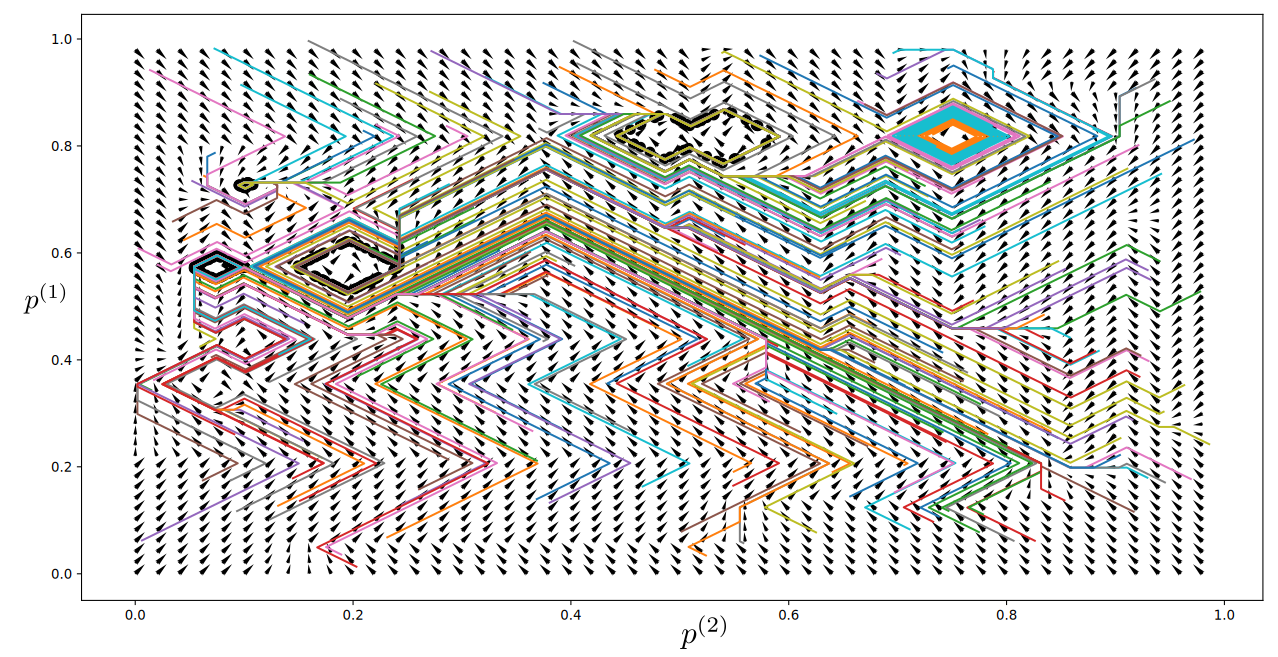
\includegraphics[width=\textwidth]{champ_006_t1.pdf}
\caption{Champ de déplacements de $\bmu\m{1}_\tau,\bmu\m{2}_\tau$ lorsque les poids sont aléatoires, à $t=0$. Nous représentons les trajectoires de 200 relaxations initialisées différemment. En fonction de la position initiale des BMUs, la relaxation évolue vers un point fixe ou un cycle limite.}
\label{fig:champ_0}
\end{figure}


\begin{figure}
\centering
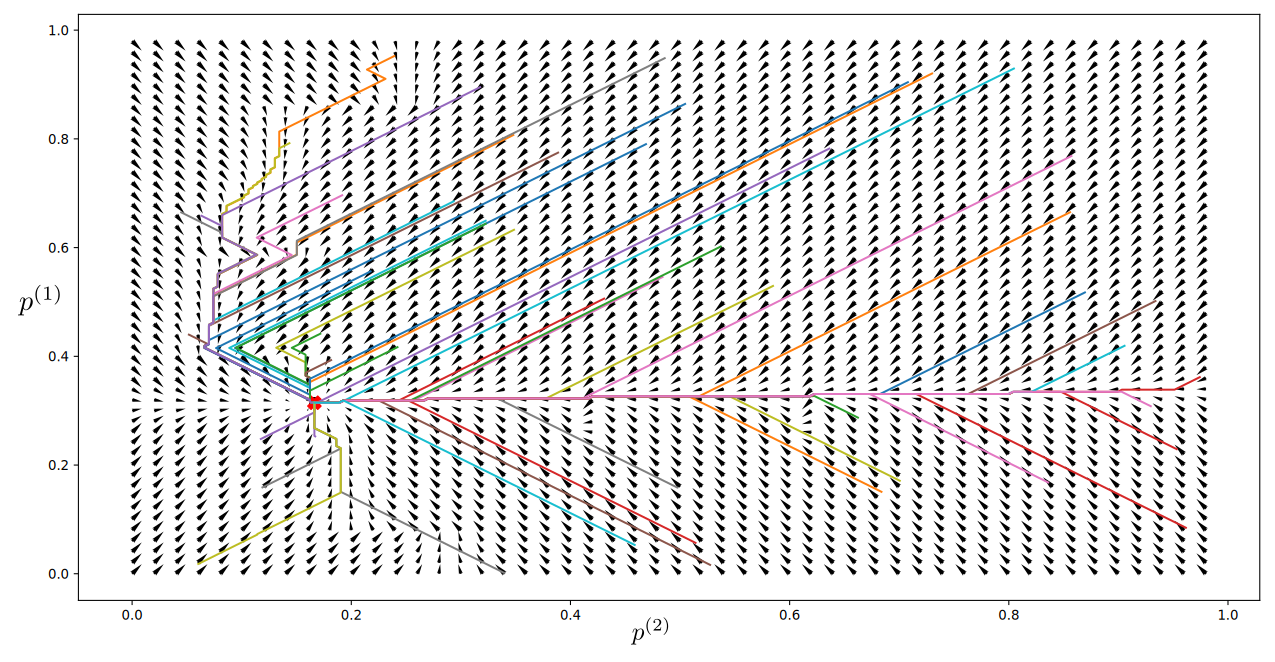
\includegraphics[width=\textwidth]{champ_006.pdf}
\caption{Champ de déplacements de $\bmu\m{1},\bmu\m{2}$ lorsque les poids sont organisés tels que représentés en figure \ref{fig:w006}, à $t=9999$. Nous y représentons les trajectoires suivient par 50 relaxations initialisées différenmment. Les relaxations évoluent vers un point fixe commun. }
\label{fig:champ_9999}
\end{figure}

\begin{figure}
	\includegraphics[width=\textwidth]{am_w_006_noinp}
	\caption{(a): $\hat{p}\m{1}$ et $\hat{p}\m{2}$ en fonction de l'entrée contextuelle de leur carte $\bmu\m{2}$ et $\bmu\m{1}$.(b): les poids externes et contextuels des cartes $1$ et $2$ sont représentés selon leur position dans la carte. On représente également les entrées test $\inpx\m{1}$ et $\inpx\m{2}$ en fonction de leur BMU. Les entrées utilisées pour tracer les figures de gauche sont colorées en rouge sur les figure de droite: $\inpx\m{1}=0.26,\inpx\m{2}=0.06$. Les intervalles dans lequel les valeurs de $\hat{p}$ varient sont reportés sur la figure (b).}
	\label{fig:w006}
	\end{figure}

\subsection{Influence du pas de relaxation}

Dans les expériences précédentes, nous avons utilisé un pas de convergence $\Delta=0.05$.
Une autre solution est de ne pas utiliser de pas de relaxation, c'est à dire, à chaque itération, déplacer le BMU $\bmu\m{i}_\tau$ directement en $\hat{p}\m{i}$, où l'activité globale est maximale, au lieu de le déplacer de $\Delta$.

L'évolution de la relaxation devient alors:
\begin{equation}
\forall i, \bmu\m{i}_{\tau+1} = \hat{p}\m{i}_{\tau}
\end{equation}

On pourrait supposer que prendre un petit $\Delta$ permet une meilleure convergence; en fait, la valeur de $\Delta$ influence peu la capacité de convergence et l'organisation des cartes.
En figure \ref{fig:diff_nopas}, nous avons tracé plusieurs trajectoires de relaxation réalisées après apprentissage,pour une même entrée. 
Nous représentosn sur cette même figure les différences $\lvert \hat{p}\m{1} - p\m{1} \rvert$ et $\lvert \hat{p}\m{2} - p\m{2} \rvert$.
La méthode de relaxation utilisée lors de l'apprentissage menant à la configuration de poids utilisée pour cette expérience n'a pas non plus utilisé de pas de relaxation $\Delta$.
A l'issue de l'apprentissage, le comportement de la relaxation ne change pas par rapport à celui observé en figure \ref{fig:diff_relax_notraj}~: les trajectoires convergent vers le point fixe de $\mathbf{f}$.
Cela se comprend au vu des résultats précédents. $\hat{p}\m{1}$ et $\hat{p}\m{2}$ sont dans un intervalle réduit de valeurs de la carte, quelles que soient les positions $p\m{1}$ et $p\m{2}$. 
Amener directement le BMU dans cet intervalle ou l'y amener pas à pas change peu le comportement de la suite. 

\begin{figure}
\begin{minipage}{0.5\textwidth}
\includegraphics[width=\textwidth]{champ_X_009}
\end{minipage}
\begin{minipage}{0.5\textwidth}
\includegraphics[width=\textwidth]{champ_Y_009}
\end{minipage}
\caption{Trajectoires des relaxations $(\bmu\m{1}_{\tau},\bmu\m{2}_\tau)$ dans le champ des différences ${\hat{p}}\m{1} - p\m{1}$ et ${\hat{p}}\m{2} - p\m{2}$, lorsque la relaxation est effectuée sans utiliser de petits déplacements. Les tracés sont effectués après apprentissage. La relaxation semble encore converger vers un point fixe.}
\label{fig:diff_nopas}
\end{figure}

% \section{Conclusion}

% Les parties \ref{sec:conv} et \ref{sec:cont} montrent donc que, lorsque les poids sont quelconques, la convergence de l'algorithme de relaxation n'est pas assurée; au contraire, la relaxation évolue dans la plupart des cas vers une situation non convergente. Dans le cas particulier étudié dans la section, il semble exister des point fixes, mais dus au caractère aléatoire des poids. La relaxation ne permet pas de trouver ces points. Pourtant, l'apprentissage des cartes utilisant la relaxation comme recherche de BMU mène une organisation des poids, même sans que la relaxation ne converge au début. Cette organisation permet de plus une meilleure convergence de la relaxation (convergence dans plus de $90 \%$ des cas).

% Ce comportement peut être expliqué. On observe que la relaxation converge bien à partir du moment où les poids externes sont organisés et présentent une continuité. 
% Au début de l'apprentissage, même si la relaxation mène à des positions quelconques de BMUs, ces BMUs auront quand même des poids externes restant proches de la valeur de l'entrée externe. 
% Le calcul de l'activité dépend en effet d'abord de l'activité externe de la carte:
% $$ a_g = \sqrt{a_e ( \beta a_e + (1-\beta a_c))}, \;\; \beta=0.5$$ 
% De plus, la relaxation est initialisée à une position correspondant au maximum de l'activité externe.

% L'organisation de la carte s'effectuera donc de façon similaire à une carte classique. Dans une carte de Kohonen, pour des poids aléatoires, de multiples positions de BMU sont possibles lors du calcul de la distance des poids à l'entrée. La disposition des poids et le choix du BMU n'influencent pas la propriété globale d'organisation d'une carte. Cette même observation peut s'effectuer ici. 
% Le rayon de voisinage externe étant bien plus grand que le rayon de voisinage contextuel, l'organisation des poids externes de la carte influence peu l'organisation des poids contextuels.
% Lorsque les poids externes présentent une continuité, la relaxation converge. Les poids contextuels peuvent alors s'organiser selon le BMU, qui a maintenant un sens: il s'agit d'un point fixe de la fonction de relaxation. Le BMU correspond alors au point qui maximise en même temps les activités globale de chaque carte.

% Expérimentalement, on observe que, lorsque les cartes sont organisés, le point fixe  existe, est unique est est atteint par n'importe quelle trajectoire de relaxation. Le BMU a donc un sens au niveau de la carte. 

% Enfin, la relaxation utilise un pas de déplacement utilisé $\delta$. 
%

% La relaxation est donc une recherche d'un maximum global à l'architecture, ce maximum étant un point fixe de la fonction de mise à jour des positions.
% Une fois que les poids externes d'une carte présentent une continuité, la relaxation et le BMU issu de ce processus ont un sens topologique: on observe expérimentalement que la fonction de mise à jour présente un point fixe $\mathbf{\bmu} = \mathbf{f}(\mathbf{\bmu})$, et que la relaxation converge vers ce point fixe. Ce point fixe est alors le point qui maximise \emph{collectivement} les activités globales de chaque carte de l'architecture.
% Bien que la relaxation ne converge pas au début de l'apprentissage, la convergence est observée dès que les poids externes présentent une certaine continuité. Cette continuité étant assurée après quelques itérations d'apprentissage par l'algorithme de mise à jours des poids de Kohonen, on peut donc dire que la relaxation converge au sein de CxSOM.


\section{Conclusion}

Ce chapitre présente une étude expérimentale du mécanisme de relaxation. Nous avons détaillé un formalisme décrivant l'algorithme, qui montre que la relaxation est une recherche du maximum de l'activation globale de l'architecture, soit la somme des activations de chaque carte.
La relaxation est alors un moyen de trouver un ensemble de BMU au sein d'une architecture maximisant une propriété \emph{globale} à cette architecture: toutes les cartes voient leur activité globale maximisée. 
Cette recherche de maximum est réalisée localement, au niveau de chaque carte, et non de façon globale. La relaxation agit alors comme une manière de connecter des cartes de façon non-hiérarchique et les BMUs sont 
l'interface entre modules de la carte.

La convergence de la relaxation dépend de la disposition des poids des cartes.
Nous avons observé expérimentalement que lorsque les poids des cartes ne sont pas ordonnés, il n'existe pas forcément de solution au problème d'optimisation. Dans ce cas, la relaxation converge seulement dans 20\% des cas lors d'une étape de test.
Cependant, nous avons observé que les cartes se déplient correctement même lorsque la relaxation n'a pas convergé,c e qui est assuré grâce à l'initialisation de la relaxation à des positions maximisant l'activité externe et grâce à la prépondérance de l'activité externe dans le calcul de l'activité globale. 
La relaxation va alors évoluer vers un point qui, même s'il n'est pas une solution du problème de maximisation globale, maximise bien l'activité externe de la carte~: $\w_e(\bmu)$ est proche de l'entrée. Cela permet de déplier correctement les poids externes. Une fois que ces poids externes sont dépliés, la relaxation ne peut évoluer que vers une zone réduite de la carte qui est définie par l'activité externe.

Enfin, nous avons observé que lorsque tous les poids sont bien dépliés, il existe une solution optimale du problème de relaxation. L'algorithme de recherche converge alors vers ce point quel que soient les conditions initiales.
Dans ce cas, la relaxation converge même en l'absence de pas de relaxation $\Delta$, c'est à dire lorsque les BMUs successifs considérés lors de la relaxation sont directement les positions maximisant l'activité de chaque carte.

Ces tracés de relaxation ont été effectués pour des cartes 1D prenant des entrées 1D, avec des cartes ayant un jeu de paramètre spécifique, avec notamment $r_e = 0.2$ et $r_c = 0.02$. 
Nous avons également observé que la relaxation converge sur des cartes 2D prenant des entrées 1D.
Dans les chapitre suivants, nous détaillerons le comportement des cartes 1D et 2D sur différentes données d'entrées et différents paramètres. Nous prendrons le soin de tracer dans ces chapitres l'évolution de la convergence de la relaxation, d'après la méthode proposée en figure~\ref{fig:conv_evolution}~; nous observerons la relaxation semble bien converger dès que les poids présentent un dépliement ordonné, ceci sur des cartes 1D prenant des entrées 1D mais également des cartes 2D prenant des entrées 2D au chapitre~\ref{chap:analyse2D}.

\ifSubfilesClassLoaded{
    \printbibliography
    %\externaldocument{../main.tex}   
}{}
\end{document}
